\chapter{System Design and Architecture}

DocBook follows a three-tier architecture: presentation (HTML templates), application (Django views and business logic), and data (SQLite or PostgreSQL). Figure~\ref{fig:architecture} illustrates the production deployment view.

\begin{figure}[htbp]
  \centering
  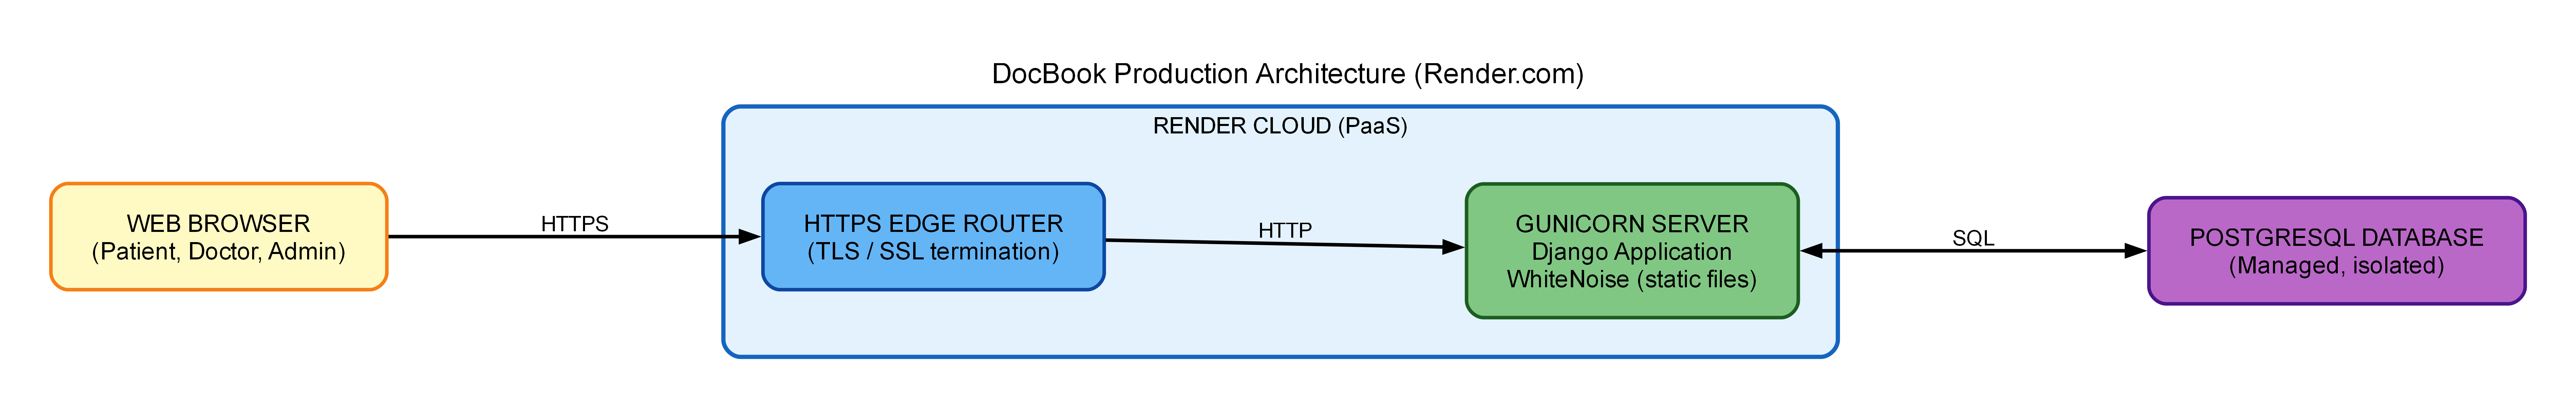
\includegraphics[width=\textwidth]{figures/docbook_architecture}
  \caption{Cloud infrastructure architecture of DocBook on Render: user traffic enters over HTTPS, is terminated at the edge router, processed by Gunicorn and Django (with WhiteNoise for static files), and persists in an isolated PostgreSQL database}
  \label{fig:architecture}
\end{figure}

\section{Database Design}

The central entity is a custom \textbf{User} model with role \texttt{doctor} or \texttt{patient}. A one-to-one \textbf{Profile} stores extended attributes. \textbf{Booking} links doctor and patient with date, time, and status; \texttt{unique\_together} on \texttt{(doctor, appointment\_date, appointment\_time)} prevents double booking. \textbf{Prescription} extends a booking one-to-one. \textbf{Review} links patient, doctor, and booking with a 1--5 rating. Figure~\ref{fig:erd} shows the entity-relationship layout generated from the Django models (\texttt{accounts}, \texttt{bookings}, \texttt{core}).

\begin{figure}[htbp]
  \centering
  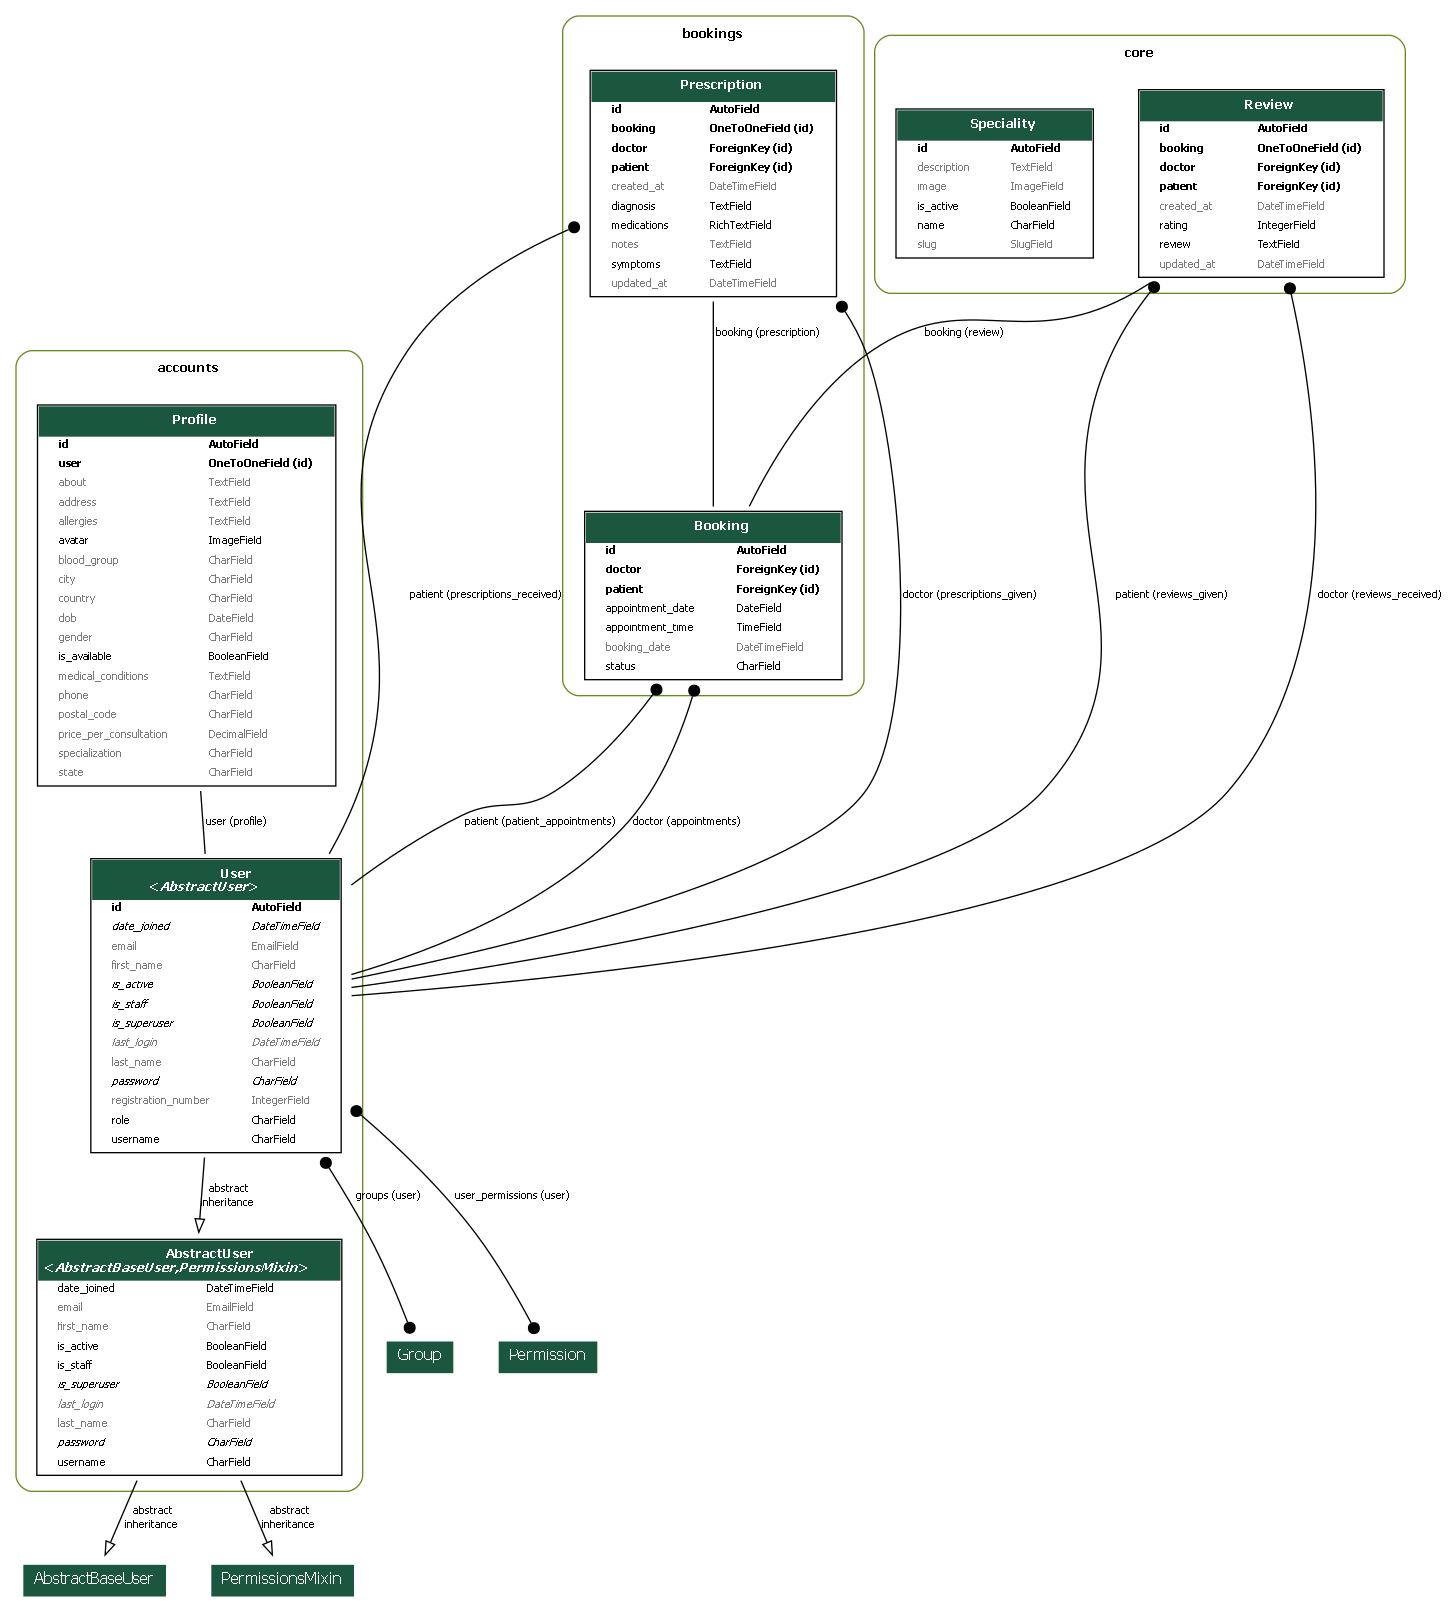
\includegraphics[width=\textwidth]{figures/docbook_erd}
  \caption{Entity-relationship diagram of DocBook core entities}
  \label{fig:erd}
\end{figure}

\section{Backend Design}

Role-based access control uses \texttt{PatientRequiredMixin}, \texttt{DoctorRequiredMixin}, and \texttt{AdminRequiredMixin}. Object-level checks ensure patients access only their own bookings. Middleware includes security, CSRF, session, and authentication layers.

\section{Frontend Design}

\subsection{Django Templates and Bootstrap}
Templates extend a common base layout. Navigation is role-specific after login.

\subsection{HTMX}
Used for partial updates on doctor profile forms without full page reload.

\subsection{jQuery and Chart.js}
jQuery supports legacy components; Chart.js renders admin dashboard statistics.

\subsection{Django REST Framework}
JSON endpoints update profile fragments where asynchronous behaviour helps.

\subsection{URL Routing Structure}
Public routes under \texttt{/}, authentication under \texttt{/accounts/}, role dashboards under \texttt{/patients/}, \texttt{/doctors/}, and \texttt{/admin/}.

\section{Use Case Diagrams}

Actors: Patient, Doctor, Administrator. Main use cases: book appointment, confirm appointment, manage schedule, view reports. (Insert diagram exported from draw.io or Word.)

\section{Wireframes and Interface Screens}

Insert screenshots of home page, login, patient dashboard, doctor schedule, booking confirmation, and admin dashboard as Figures in this section. See Appendix for the full list.
